
\section{Results}
\label{sec:results}

\subsection{Data Status}

All results reported in this section were generated using
synthetic data for pipeline validation. They do not constitute
empirical evidence about students or AI-companion users.
The synthetic dataset contains 171 observations.

\subsection{RQ2: Emotional-Dependence Marker Frequency}
\label{subsec:rq2-results}

Table~\ref{tab:rq2-summary} summarizes the synthetic
emotional-dependence marker frequencies across three
engagement-duration groups.

\begin{table}[t]
\centering
\caption{Synthetic RQ2 Group Summary (Pipeline Test Only)}
\label{tab:rq2-summary}
\begin{tabular}{lrrr}
\toprule
Duration & $n$ & Median & IQR \\
\midrule
$<1$ month   & 38 & 10.69 & 9.58 \\
1--3 months  & 57 & 11.70 & 12.02 \\
$>3$ months  & 76 & 20.78 & 23.93 \\
\bottomrule
\end{tabular}
\end{table}

The highest median was observed in the synthetic
long-duration group ($>3$ months).

Figure~\ref{fig:rq2-boxplot} displays the synthetic
author-level distributions behind this comparison.


\begin{figure}[t]
  \centering
  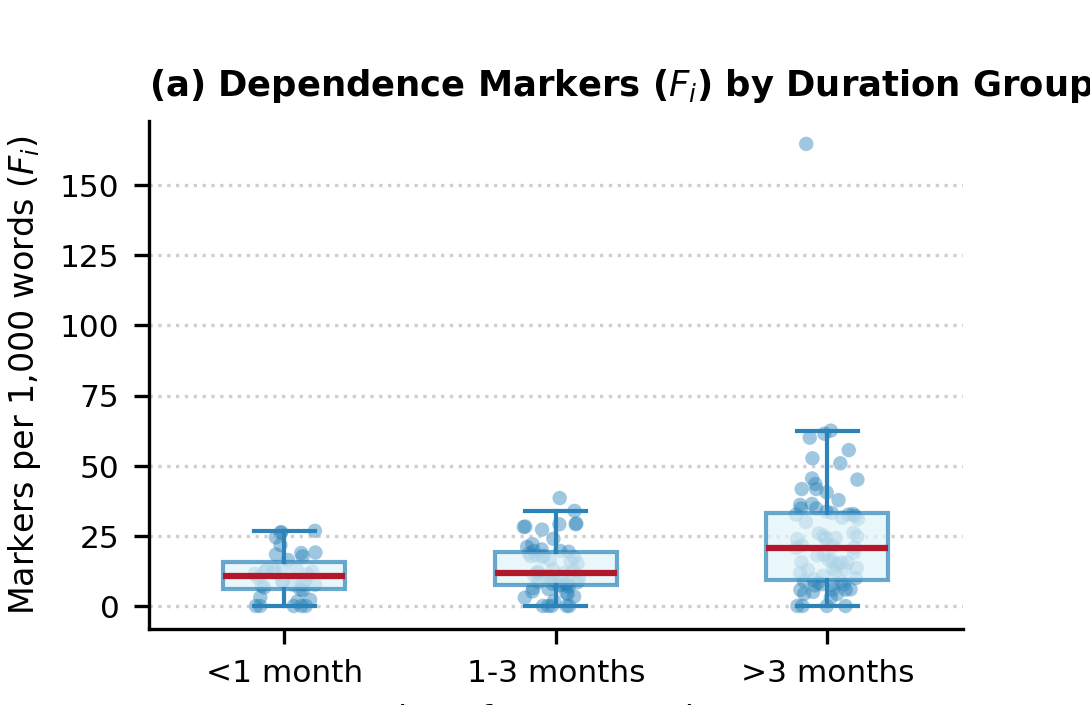
\includegraphics[width=\columnwidth]
    {figures/rq2_boxplot.png}
  \caption{Synthetic emotional-dependence marker
  rates by engagement duration.
  Pipeline validation only.}
  \label{fig:rq2-boxplot}
\end{figure}


The one-sided Mann--Whitney $U$ test comparing the
long-duration and short-duration groups yielded
$U=2079.5$ and $p<0.001$.
Cliff's $\delta$ was 0.440, with a bootstrap
95\% confidence interval of [0.250, 0.614].

The Kruskal--Wallis test across the three groups
yielded $H=19.147$ ($p<0.001$).
The Jonckheere--Terpstra trend test produced
a statistic of 6206.5 ($Z=4.354$, $p<0.001$).

These statistics demonstrate the behavior of the
analysis pipeline on synthetic inputs rather than
substantive findings about human behavior.

\subsection{RQ3: Social-Avoidance Indicators}
\label{subsec:rq3-results}

In the synthetic dataset, Spearman's rank correlation
between engagement duration and the social-avoidance
index was $\rho=0.136$ ($p=0.038$, one-sided).

The correlation between weekly session frequency and
the social-avoidance index was $\rho=0.082$
($p=0.144$, one-sided).

In the OLS model specified in
Eq.~\eqref{eq:rq3-model}, controlling for weekly
session frequency, the duration coefficient was
$\beta_1=-0.129$ ($p=0.645$), while the
session-frequency coefficient was
$\beta_2=-0.619$ ($p=0.278$).

The model explained approximately 0.8\% of the
variation in the synthetic outcome
($R^2=0.008$).

Table~\ref{tab:baseline-comparison} compares
the unadjusted correlation baseline with the
covariate-adjusted analysis on the same
synthetic observations. The coefficients
represent different estimands and are not
directly comparable.

\begin{table}[t]
\centering
\caption{Synthetic RQ3 Baseline Comparison}
\label{tab:baseline-comparison}
\begin{tabular}{lcc}
\toprule
Metric & Spearman & Adjusted OLS \\
\midrule
Duration effect & $\rho=0.136$ & $\beta=-0.129$ \\
$p$-value & 0.038 & 0.645 \\
Controls sessions & No & Yes \\
Observations & 171 & 171 \\
\bottomrule
\end{tabular}
\end{table}


Thus, the weak positive unadjusted correlation
was not reflected in a statistically significant
adjusted duration coefficient.
No substantive inference about real users
can be drawn from these synthetic results.
